%%%%%%%%%%%%%%%%%%%%%%%%%%%%%%%%%%%%%%%%%%%%%%%%%%%%%%%%%%%%%%%%%%%%%%%%%
\section{Introduction} 
\label{sec:introduction}

Sign language is a visual communication skill that enables individuals with different types of hearing impairment to communicate in society. It is the language used by most deaf people in their daily lives and, moreover, it is the symbol of identification between the members of that community and the main force that unites them~\cite{pereira-choi-2011}. % It has a very close relationship with the culture of the country or even regions, and for this reason, each nation has its sign language~\cite{pereira-choi-2011}.

According to the World Health Organization, the number of people with disabling hearing loss is about 360 million, which is equivalent to a forecast of 1 in 10 individuals around the world~\cite{who-2018}. This data, in turn, highlight the breadth and importance of sign language in the communication of many of these people.

Despite this, there is still a small number of hearing people able to communicate through sign language. This ends up characterizing an invisible barrier that interferes with the communication between deaf and hearing persons, making a more effective integration among these people impossible~\cite{peres-2006}. In this context, it is essential to develop tools that can fill this gap by promoting integration among the population.

Research related to the sign recognition have been developed since the 1990s, and it is possible to verify significant results~\cite{lim-2016,recent-advances-dl-2017}. The main challenges are primarily related to considering the dynamic aspects of the language, such as movements, articulations between body parts and non-manual expressions, rather than merely recognizing static signs or isolated hand positions. % Besides, the sign language has thousands of signs, which sometimes differ only by subtle changes in movement, shape, or position of the hands and involve significant overlaps of fingers and occlusions. When combined with differences in signing style by distinct individuals and the variations arising from its non-universality and regionalisms, this field of research can become challenging for current artificial intelligence algorithms~\cite{konstantinidis-2018}.

In this work, we present a new approach to performing the recognition of human actions based on spatial-temporal graphs called Spatial-Temporal Graph Convolutional Networks (ST-GCN) \cite {st-gcn-2018}. Using graph representations of the human skeleton we focus on body movement and the interactions between its parts, disregarding the interference of the environment around them. Besides, we address the movements under the spatial and temporal dimensions, and this allows us to capture the dynamic aspects of the actions exercised over time. These characteristics make it a very relevant approach to dealing with the challenges and peculiarities of sign language recognition.
 
% To develop the proposed method, however, it is first necessary to build a dataset of human skeletons associated with sign language that would serve as the primary information to feed the ST-GCN and enable the creation of its graphs. We used as a base the videos of the American Sign Language Lexicon Video Dataset (ASLLVD). It consists of a large set of the American Sign Language (ASL), on which we perform segmentation and assignment of estimated skeleton labels. 

The main contributions of the paper are: 1) the proposition of a new technique to sign recognition based on human movement, which considers different aspects of its dynamics and contributes to overcoming some of the main field challenges; and 2) the creation of a new dataset of human skeletons for sign language, currently non-existent, which aims to support the development of studies in this area.

Section~\ref{sec:related-work} presents the related works and the details of ST-GCN. In Section~\ref{sec:new-dataset},  the creation of the new database is discussed.
Section~\ref{sec:st-gcn-for-sl-recognition} addresses the adjustments in ST-GCN and Section~\ref{sec:experiments} the conduction of the experiments. Finally, Sections~\ref{sec:results}~and~\ref{sec:final-remarks} contains the results and final remarks respectively. \\[-8mm]

%%%%%%%%%%%%%%%%%%%%%%%%%%%%%%%%%%%%%%%%%%%%%%%%%%%%%%%%%%%%%%%%%%%%%%%%%
\section{Related work}
\label{sec:related-work}

The recognition of sign languages obtained significant progress in recent years, which are motivated mainly by the advent of modern sensors, new machine learning techniques, and more powerful hardware~\cite{recent-advances-dl-2017,recent-advances-sl-2013}. Besides, approaches considered intrusive and requiring the use of sensors such as gloves, accelerometers, and markers coupled to the body of the interlocutor have been gradually abandoned, replaced by new approaches using conventional cameras and computer vision techniques.

Due to this movement, it is also notable the increase in the adoption of techniques for feature extraction such as SIFT, HOG, HOF and STIP to preprocess the images obtained by cameras and provide richer information to machine learning algorithms~\cite{laptev-2008,lim-2016,shanta-2018}.

Convolutional Neural Networks (CNN), as in many computer vision applications, obtained remarkable results in this field with accuracy reached 90\% depending on the dataset \cite{shanta-2018,taskiran-2018,rao-2018}. There are still some variations as 3D CNNs~\cite{elbadawy-2017}, the combination with other models such as Inception~\cite{das-2018} or the Regions of Interest applications~\cite{sajanraj-2018}. Recurrent Neural Networks~\cite{konstantinidis-2018} and Temporal Residual Networks~\cite{pigou-2017} also obtained interesting results in the same purpose.

Despite the above advances, a large portion of these studies addresses static signs or single-letter images, from the dactylology\footnote{Dactylology - digital or manual alphabet, generally used by the deaf to introduce a word that does not yet have an equivalent sign~\cite{pereira-choi-2011}.
}~\cite{taskiran-2018,elbadawy-2017,das-2018}. The problem is the negative effects on the intrinsic dynamics of the language, such as its movements, non-manual expressions, and articulations between parts of the body~\cite{quadros-2004}. In this sense, it is extremely relevant that new studies observe such important characteristics.

With this purpose, we present an approach based on skeletal body movement to perform sign recognition. This technique is known as Spatial-Temporal Graph Convolutional Network (ST-GCN)\footnote {Available at \url{https://github.com/yysijie/st-gcn}.} and was introduced in~\cite{st-gcn-2018}. The approach aims for methods capable of autonomously capturing the patterns contained in the spatial configuration of the body joints as well as their temporal dynamics. % The authors suggest that previous methods for action recognition were limited by not explicitly exploring such spatial relations between the joints, which are crucial for the understanding of human actions. These methods simply used the joint coordinates in individual time steps to form feature vectors, applying a temporal analysis on them~\cite{st-gcn-2018,wang-2012,fernando-2015}.

The ST-GCN uses as a base of its formulation a sequence of skeleton graphs representing the human body obtained from a series of action frames of the individuals. Figure~\ref{fig:st-gcn-graph} allows to visualizing this structure, where each node corresponds to an articulation point. The intra-body vertices are defined based on the body's natural connections. The inter-frame vertices, in turn, connect the same joints between consecutive frames to denote their trajectory over time~\cite{st-gcn-2018}. \\[-8mm]
    

\begin{figure}
    \centering
    \begin{subfigure}{.30\textwidth}
        \centering
        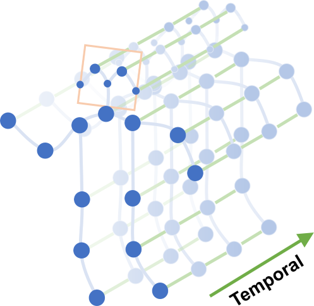
\includegraphics[height=2.7cm]{images/st_gcn_graph}
        \caption{}
        \label{fig:st-gcn-graph}
    \end{subfigure}
    \begin{subfigure}{.30\textwidth}
      \centering
      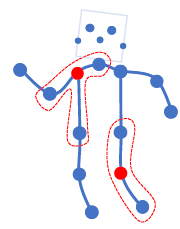
\includegraphics[height=2.7cm]{images/st_gcn_sampling}
      \caption{}
      \label{fig:st-gcn-sampling}
    \end{subfigure}
    \begin{subfigure}{.30\textwidth}
      \centering
      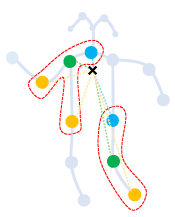
\includegraphics[height=2.7cm]{images/st_gcn_spatial_partitioning}
      \caption{}
      \label{fig:st-gcn-spatial-part}
    \end{subfigure}
    \caption{
        (\subref{fig:st-gcn-graph})~Sequence of skeleton graphs, denoting human movement in space and time. 
        (\subref{fig:st-gcn-sampling})~Sampling strategy in a convolution layer for a single frame.
        (\subref{fig:st-gcn-spatial-part})~Spatial Configuration Partitioning strategy \cite{st-gcn-2018}.
    }
    \label{fig:graph_part_sampling}
\end{figure}    

\vspace{-5mm}   
    
%\image
%    [3.0cm]
%    {fig:st-gcn-graph}
%    {images/st_gcn_graph}
%    {Sequence of skeleton graphs, denoting human movement in space and time, used by the ST-GCN \cite[p. 1]{st-gcn-2018}.}

Figure \ref{fig:st-gcn-workflow} gives an overview of this technique. First, the estimation of individuals' skeletons in the input videos, as well as the construction of space-time graphs based on them. Then, multiple ST-GCN convolution layers are applied, gradually generating higher and higher levels of feature maps for the presented graphs. Finally, they are submitted to a classifier to identify the corresponding action.

To understand the operation of the ST-GCN, it is necessary first to introduce its sampling and partitioning strategies. When we are dealing with convolutions over 2D images, it is easy to imagine the existence of a rigid grid (or rectangle) around a central point that represents the sampling area of the convolutional filter, which delimits the neighborhood. In the case of graphs, however, it is necessary to look beyond this definition and consider the neighborhood of the center point as points that are directly connected by a vertex. Figure \ref{fig:st-gcn-sampling} represents this definition for a single frame. Note that for the red center points, the dashed edges represent the sampling area of the convolutional filter. Note also that although there are other points physically close to the central points (such as the points of the feet, knees, and waist), the method does not consider this points unless there is a vertex connecting them to the red points. This sequence of steps is the \textbf{sampling strategy} of ST-GCN. \\[-8mm]

%\image
%    [2.5cm]
%    {fig:st-gcn-sampling}
%    {images/st_gcn_sampling}
%    {Sampling strategy in a convolution layer for a single frame \cite[p. 5]{st-gcn-2018}.}


\begin{figure*}[!ht]
    \centering
    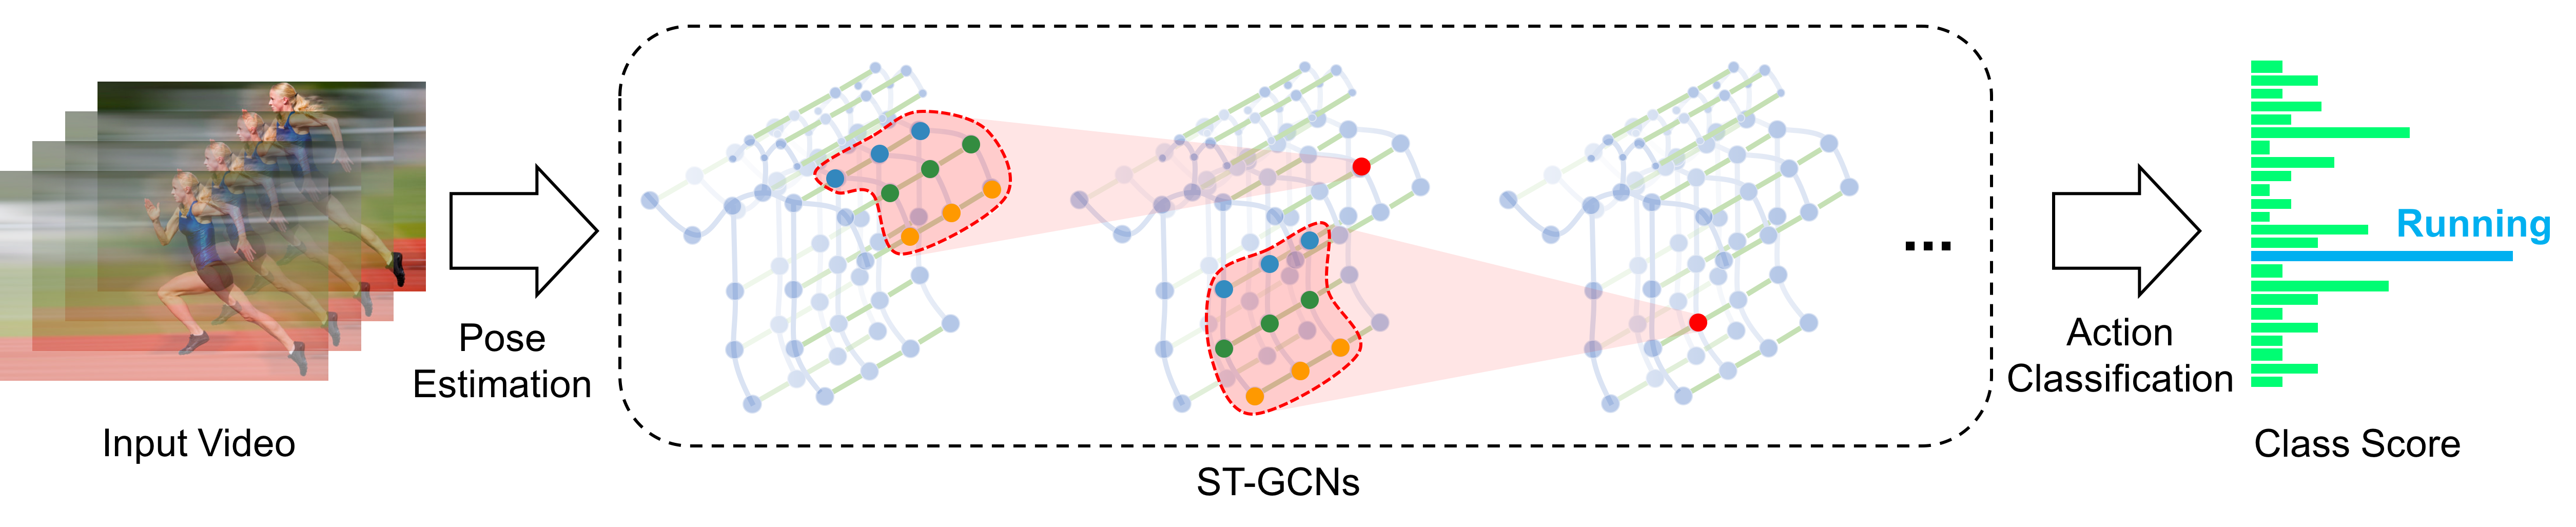
\includegraphics[width=1.0\textwidth]{images/st_gcn_workflow}
    \caption{Overview of the ST-GCN approach \cite[p. 3]{st-gcn-2018}.}
    \label{fig:st-gcn-workflow}
\end{figure*}

\vspace{-5mm}

Figure~\ref{fig:st-gcn-sampling} shows how the convolutional filter considers only points immediately connected to the central points. In other words, the delimitation of the filter area consider the neighbors with distance $D = 1$. The authors defined this distance in ST-GCN proposition paper \cite{st-gcn-2018}. 

The \textbf{partitioning strategy} is based on the location of the joints and the characteristics of the movement of the human body, as shown in Figure~\ref{fig:st-gcn-spatial-part}. According to the authors, concentric or eccentric movements categorize the body parts, and the points in the sampling region are partitioned into three subsets: %\\[-5mm]
    
\begin{itemize}
    \item The root node (or center point, marked green in Figure~\ref{fig:st-gcn-spatial-part});
    \item The centripetal group (blue dots in the Figure~\ref{fig:st-gcn-spatial-part}), which are the neighborhood nodes that are closest to the center of gravity of the skeleton (black cross);
    \item The centrifugal group (yellow dots in the Figure~\ref{fig:st-gcn-spatial-part}), which are the nodes farther from the center of gravity.
\end{itemize}

The center of gravity is taken to be the average coordinate of all joints of the skeleton in one frame. During convolution, each point of the body is labeled according to one of the above partitions named Spatial Configuration Partitioning~\cite{st-gcn-2018}. It is through this method that the authors also establish the weights of the model, making each of the partitions receive a different weight to be learned.

%\image
%    [2.5cm]
%    {fig:st-gcn-spatial-part}
%    {images/st_gcn_spatial_partitioning}
%    {Spatial Configuration Partitioning strategy \cite[p. 5]{st-gcn-2018}.}
    
% In order to learn the temporal dimension, the ST-GCN extends the concept of graph convolution shown above to the scheme presented in the Figure~\ref{fig:st-gcn-convolution}.
In order to learn the temporal dimension, the ST-GCN extends the concept of graph convolution shown above, considering this dimension as a sequence of skeletons graphs stacked consecutively, as in Figure~\ref{fig:st-gcn-graph}. With this, we have in hands a set of graphs that are neighbors to each other. Let us now assume that each articulation of the body in a graph must be connected using a vertex to itself in the graph of the previous neighbor frame and also in the next neighbor frame. Given that, if we return to the definition of sampling introduced above, we verify that the convolutional filter contemplates those points belonging to the neighboring graphs, that now fit the requirements of being directly connected at a distance $D = 1$. In this way, ST-GCN considers the spatial and temporal dimensions and applies convolutions on them.

% \image
%    [8.0cm]
%    {fig:st-gcn-convolution}
%    {images/st_gcn_convolution}
%    {Convolution on the spatial and temporal dimensions, which considers the points directly connected in the current and neighboring graphs \cite[p. 3]{st-gcn-2018}.}

% Figure~\ref{fig:st-gcn-architecture} (left) shows the model architecture and its convolutional layers, according to~\cite{st-gcn-2018}. There are a total of nine sequentially positioned ST-GCN layers, which perform the extraction of features from the graphs. A normalization layer preceded them and followed by a global pooling and a softmax classification layer. On the right side of the image, we also show the details of an ST-GCN convolutional unit.

%\begin{figure}[ht]
%    \centering
%    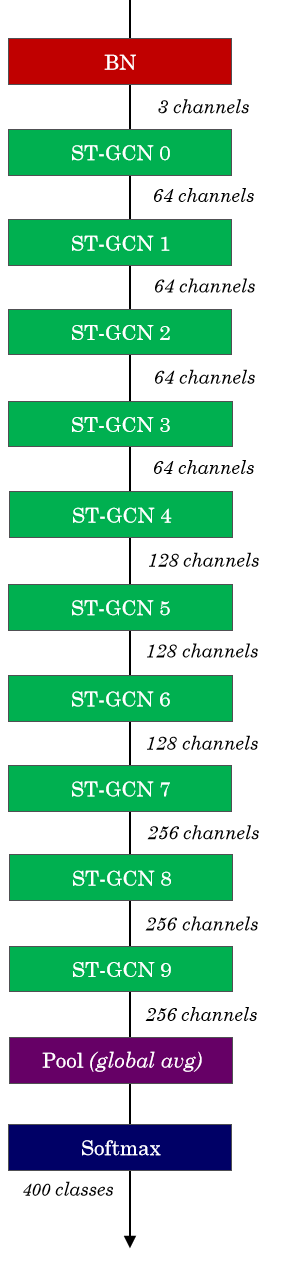
\includegraphics[width=2.5cm]{images/st_gcn_architecture}
%    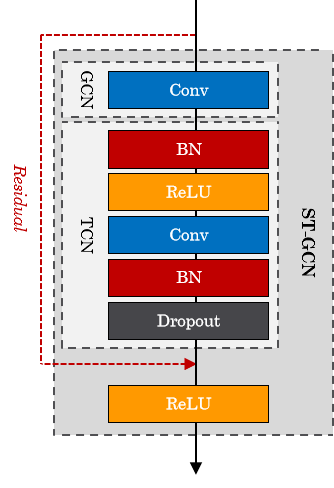
\includegraphics[width=3.0cm]{images/st_gcn_architeture_unit}
%    \caption{ST-GCN Model architecture (left) and details of one convolutional unit (right). Image adapted from~\cite{st-gcn-2018}.}
%    \label{fig:st-gcn-architecture}
%\end{figure}

To estimate the skeletons of individuals in videos, the authors~\cite{st-gcn-2018} used a library called OpenPose. It is an open-source tool that uses deep learning algorithms to detect and estimate up to 130 human body points, as presented in~\cite{cao-realtime-2017,simon-hand-2017,wei-cpm-2016}. \\[-8mm]
% as shown in Figure~\ref{fig:keypoints-openpose}, and presented in~\cite{cao-realtime-2017,simon-hand-2017,wei-cpm-2016}.

%\begin{figure}[ht]
%    \centering
%    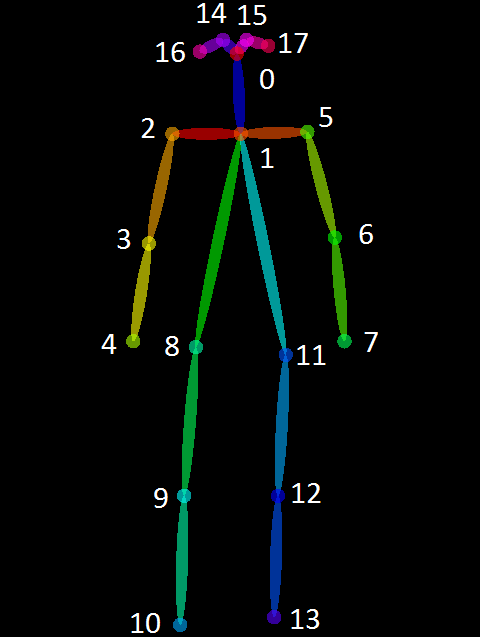
\includegraphics[width=2.5cm]{images/keypoints_pose_COCO_18}
%    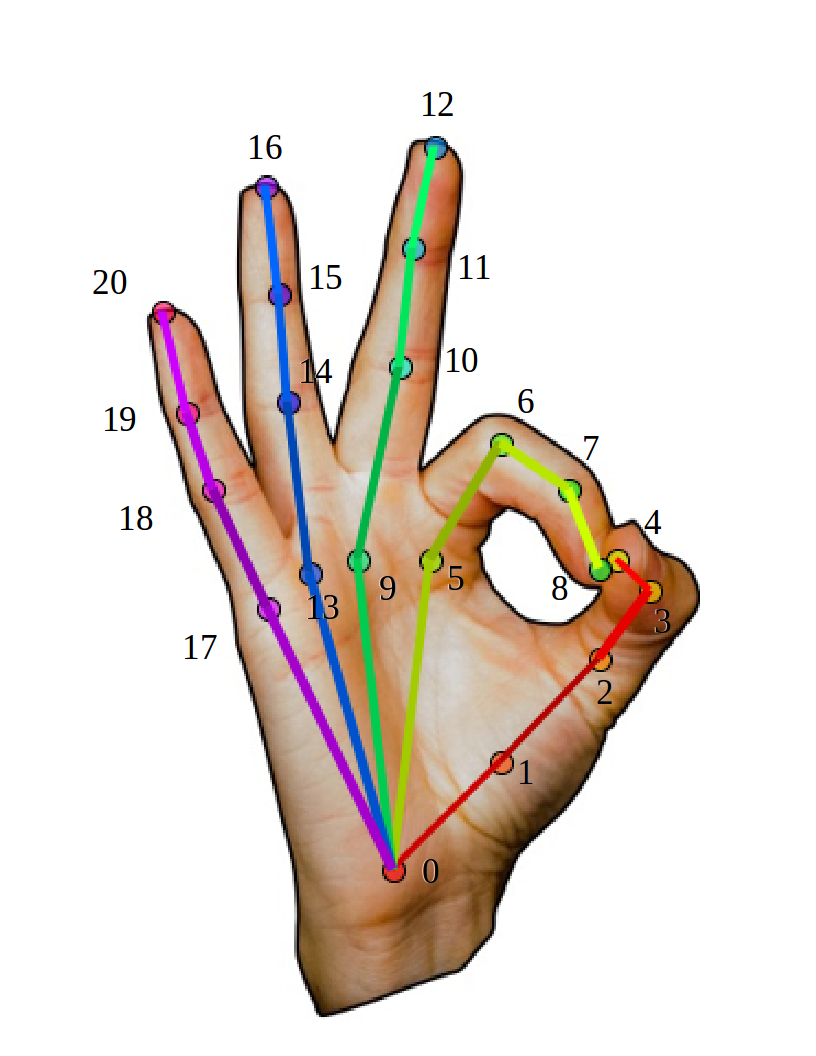
\includegraphics[width=2.5cm]{images/keypoints_hand}
%    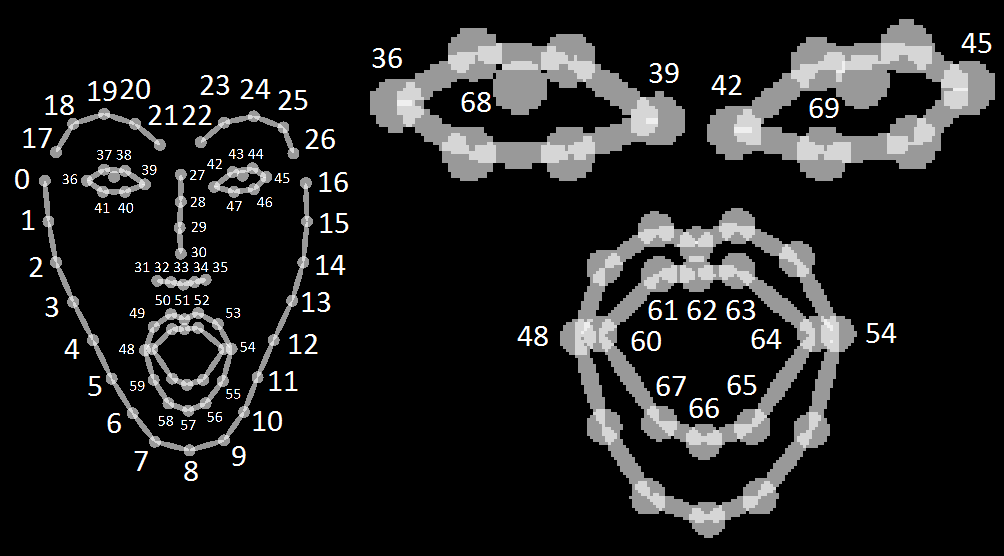
\includegraphics[width=3cm]{images/keypoints_face}
%    \caption{Representation of the 130 points estimated by OpenPose, 18 correspond to the body (left); 21 correspond to each of the hands (center); and 70 points correspond to the face (right)~\cite{openpose-output-2018}.}
%    \label{fig:keypoints-openpose}
%\end{figure}


%%%%%%%%%%%%%%%%%%%%%%%%%%%%%%%%%%%%%%%%%%%%%%%%%%%%%%%%%%%%%%%%%%%%%%%%%
\section{New dataset of human skeletons for sign language} 
\label{sec:new-dataset}

We introduce a new dataset of human skeletons for sign language based on the American Sign Language Lexicon Video Dataset (ASLLVD). The ASLLVD  is a broad public dataset\footnote{ Available at \url{http://csr.bu.edu/asl/asllvd/annotate/index.html}.} containing video sequences of thousands of American Sign Language (ASL) signs, as well as their annotations, respective start, and end frame markings, and class labels for each sample~\cite{athitsos-asllvd-2008,neidle-2012}.

According to the authors, each sign in ASLLVD is articulated by native individuals in ASL, and video sequences are collected using a four-camera system that simultaneously captures two frontal views, one side view and one enlarged view of the face of these individuals. % Figure~\ref{fig:asllvd-example} exemplifies capturing three of these views for the "MERRY-GO-ROUND" sign. 

%\image
%    {fig:asllvd-example}
%    {images/asllvd_example}
%    {Example of the sign "MERRY-GO-ROUND" from three different perspectives, in the ASLLVD \cite[p. 2]{athitsos-asllvd-2008}.}
    
% The number and type of signs included in ASLLVD are similar in scale and scope to the set of lexical entries in existing English-to-ASL dictionaries. There is at least one example of video per sign for almost all those contained in the Gallaudet Dictionary of American Sign Language~\cite{athitsos-asllvd-2008,gallaudet-2005}.

There is a total of 2,745 signs, represented in approximately 10 thousand samples. Each sign contains between 1 and 18 samples articulated by different individuals (the average number of samples per sign is 4).

% To make the ASLLVD samples compatible with the input of the ST-GCN model, it was first necessary to apply a series of preprocessing steps, as shown in Figure~\ref{fig:preprocessamento}. These steps gave rise to a new dataset containing the estimate of the skeletons for all the signs contained therein.

To make the ASLLVD samples compatible with the input of the ST-GCN model, it was necessary to apply a series of preprocessing steps, as shown in Figure~\ref{fig:preprocessamento}. These steps, in turn, gave rise to a new dataset consisting of the skeletal estimates for all the signs contained therein, which was named \textbf{ASLLVD-Skeleton}\footnote{
   Available at \url{http://www.cin.ufpe.br/~cca5/asllvd-skeleton}}. \\[-8mm]

\begin{figure*}[ht!]
    \centering
    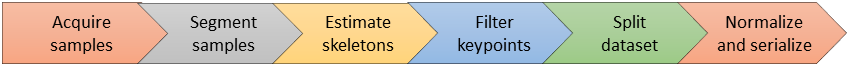
\includegraphics[width=0.9\textwidth]{images/dataset_preprocessing_en}
    \caption{Preprocessing steps for creating the ASLLVD-Skeleton dataset.}
    \label{fig:preprocessamento}
\end{figure*}

\vspace{-4mm}
% The new skeleton dataset was named \textbf{ASLLVD-Skeleton} and is public available\footnote{
%   Available at \url{http://www.cin.ufpe.br/~cca5/asllvd-skeleton}
%} to contribute to the development of future studies on the recognition of sign languages.

The first step consists of \textbf{obtaining the videos} based on the associated metadata file used to guide this process. We consider only the videos captured by the frontal camera, once they simultaneously contemplate movements of the trunk, hands, and face of the individuals.

The next step is to \textbf{segment the videos} to generate a video sample for each sign. Once every file in the original dataset corresponds to multiple signs per individual, it is necessary to change this organization in such a way that each sign is arranged individually with its respective label. % We also considered the metadata file which contains the labels and the start and end frame marks to perform the segmentation for each sign. 
The output of this step consists of small videos with a few seconds. %, as shown in Figure~\ref{fig:sign-original}.

%\image
%    [4cm]
%    {fig:sign-original}
%    {images/sign_original}
%    {Representation of the "EXAGGERATE" sign, segmented from ASLLVD dataset.}

The third step consists of \textbf{estimating the skeletons} of the individuals present in the segmented videos. In other words, the coordinates of the individuals' joints are estimated for all frames, composing the skeletons that can be used to generate the graphs of the ST-GCN method. As in \cite {st-gcn-2018}, we used the OpenPose library in this process, and a total of 130 key points were estimated. Figure~\ref{fig:sign-pose} illustrates the reconstruction in a 2D image of the estimated coordinates for the "EXAGGERATE" sign. \\[-8mm]

%\begin{figure}[ht]
%    \centering
%    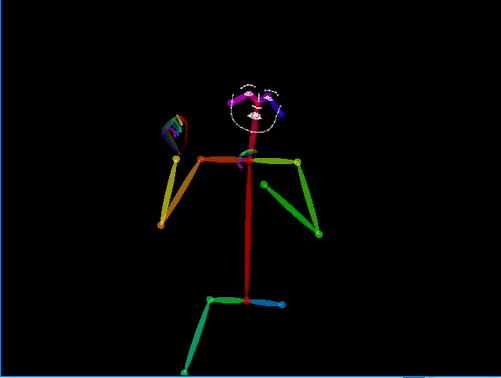
\includegraphics[width=3.5cm]{images/sign_pose}
%    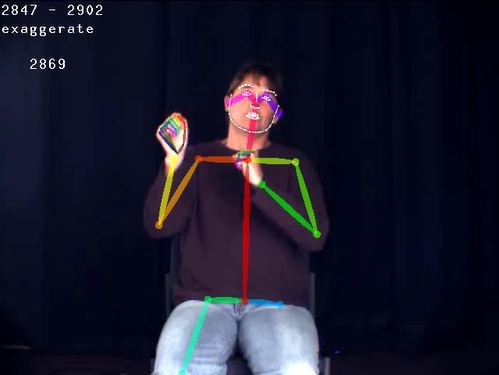
\includegraphics[width=3.5cm]{images/sign_pose_blended}
%    \caption{Reconstruction of the skeleton from the coordinates estimated by OpenPose for the sign "EXAGGERATE" (left); and the overlaping this skeleton in the original video (right).}
%    \label{fig:sign-pose}
%\end{figure}

\begin{figure}
    \centering
    \begin{subfigure}{3.5cm}
        \centering
        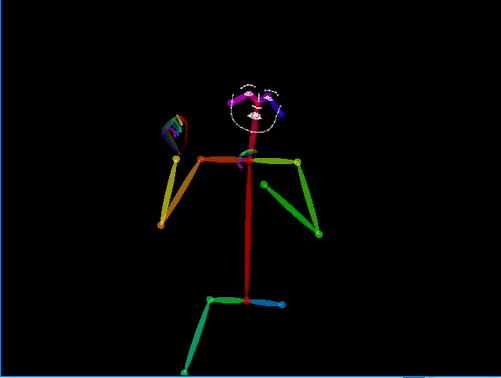
\includegraphics[width=3.5cm]{images/sign_pose}
        \caption{}
        \label{fig:sign-pose-skeleton}
    \end{subfigure}
    \begin{subfigure}{3.5cm}
      \centering
      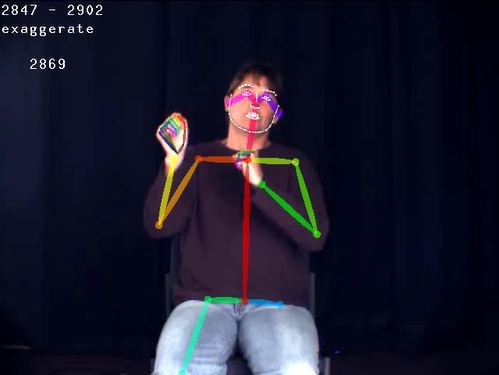
\includegraphics[width=3.5cm]{images/sign_pose_blended}
      \caption{}
      \label{fig:sign-pose-blended}
    \end{subfigure}
    \caption{
        Reconstruction of the skeleton from the coordinates estimated by OpenPose for the sign "EXAGGERATE"~(\subref{fig:sign-pose-skeleton}); and the overlaping this skeleton in the original video~(\subref{fig:sign-pose-blended}).
    }
    \label{fig:sign-pose}
\end{figure}

\vspace{-4mm}
% Figure~\ref{fig:openpose-coordinates} shows the content of an example file obtained at the end of this step. Each frame contains a section called "pose" with the coordinates of the X and Y axes estimated for the body joints, and a section "score" with the degree of confidence for each of these joints.

%\image
%    [7.5cm]
%    {fig:openpose-coordinates}
%    {images/openpose_coordinates}
%    {Example containing the estimated coordinates for the skeletons in a sign.}
    
The fourth step involves \textbf{filtering the key points}. We use only 27 of the 130 estimated key points, which 5 refer to the shoulders and arms, and 11 refer to each hand, as illustrated in Figure \ref{fig:filtered-keypoints}. \\[-8mm]% The output of this step consists of the same files as shown in Figure \ref{fig:openpose-coordinates}, but with a smaller number of coordinates per frame.

%\begin{figure}[ht]
%    \centering
%    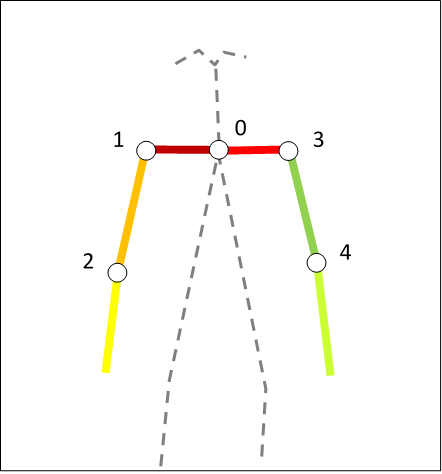
\includegraphics[height=3.2
%    cm]{images/filtered_keypoints_body}
%    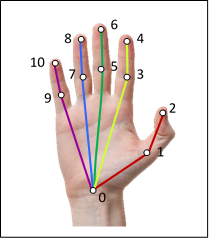
\includegraphics[height=3.2cm]{images/filtered_keypoints_hand}
%    \caption{Representation of the 27 used key points, which 5 refer to the shoulders and arms (left) and 11 refer to each hand (right).}
%    \label{fig:filtered-keypoints}
%\end{figure}


\begin{figure}
    \centering
    \begin{subfigure}{3.0cm}
        \centering
        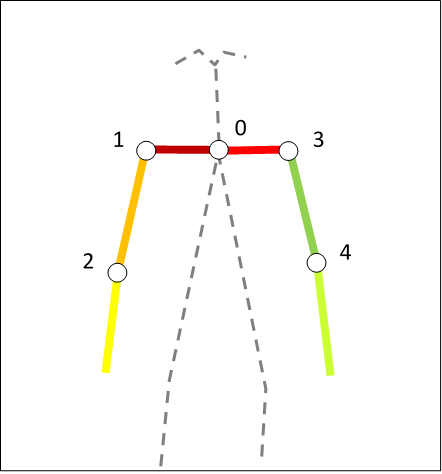
\includegraphics[height=3.2cm]{images/filtered_keypoints_body}
        \caption{}
        \label{fig:filtered-keypoints-body}
    \end{subfigure}
    \begin{subfigure}{3.0cm}
      \centering
      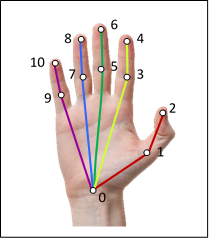
\includegraphics[height=3.2cm]{images/filtered_keypoints_hand}
      \caption{}
      \label{fig:filtered-keypoints-hand}
    \end{subfigure}
    \caption{
        Representation of the 27 used key points, which 5 refer to the shoulders~(\subref{fig:filtered-keypoints-body}) and arms and 11 refer to each hand~(\subref{fig:filtered-keypoints-hand}).
    }
    \label{fig:filtered-keypoints}
\end{figure}

\vspace{-4mm}

The fifth step concerns the \textbf{division of the dataset} into smaller subsets for training and test. For this procedure, a cross-validation dataset tool called "\textit{train\_test\_split}", available by the Scikit-Learn~\cite{scikit-learn} library was used. In this division, we assign a proportion of 80\% of the samples for training (corresponding to 7,798 samples) and 20\% for tests (corresponding to 1,950 samples). This division is a commonly adopted proportion, and we understand that the number of samples in these groups is sufficient to validate the performance of most machine learning models.

Finally, the sixth step is to \textbf{normalize and serialize} the samples to make compatible with the ST-GCN format. Normalization aims to make the length of all samples uniform by applying the repetition of their frames sequentially to the complete filling of an established fixed number of frames. The number of fixed frames adopted here is 63 (using a rate of 30 FPS, corresponds to a video with an approximate duration of 2 seconds). Serialization, in turn, consists of preloading the normalized samples from the subsets to translate them into physical Python files which contain their in-memory representations, as in ST-GCN \cite{st-gcn-2018}. We adopted this format to optimize the data loading process. % For each subset, we generate two physical files, the samples, and the labels.

The source code that performs these steps is also available in the ASLLVD-Skeleton download area$^4$.\\[-8mm]


%%%%%%%%%%%%%%%%%%%%%%%%%%%%%%%%%%%%%%%%%%%%%%%%%%%%%%%%%%%%%%%%%%%%%%%%%
\section{ST-GCN for sign language recognition} 
\label{sec:st-gcn-for-sl-recognition}

Since the graph representation approach adopted by the ST-GCN is very flexible, it is not necessary to make modifications in the architecture of the model. Instead, only punctual adaptations to consider the new coordinates of the sign language domain.

The first one is to modify the algorithm to make it able to use new customized layouts of graphs beyond those originally defined in~\cite{st-gcn-2018}. Thus, a new type of layout called "custom" was defined in the configuration file of the model. In addition, a new parameter called "custom\_layout" has been created within the "graph\_args" attribute to allow the number of nodes, the central node, and the edges of new graphs to be informed.

Once this configuration is established, it is possible to map the topology of the graph used in this paper, which is composed of the 27 joints and vertices shown in  Figure~\ref{fig:filtered-keypoints}. Finally, small adjustments were required in the dimensions of the matrices used by the data feeders and also in the file
that define the graph domain of the model so that they can now support layouts with dynamic dimensions.

The source code containing these adaptations is public available\footnote{
    Available at \url{http://www.cin.ufpe.br/~cca5/st-gcn-sl}
}. It consists of a \textit{forked} repository created from the one developed by the authors in~\cite{st-gcn-2018}. \\[-8mm]


%%%%%%%%%%%%%%%%%%%%%%%%%%%%%%%%%%%%%%%%%%%%%%%%%%%%%%%%%%%%%%%%%%%%%%%%%
\section{Experiments} 
\label{sec:experiments}

We used as reference the experiments proposed in~\cite{lim-2016}, which evaluate the performance of models as the Block-Based Histogram of Optical Flow (BHOF) (see section \ref{sec:related-work}) and also popular techniques such as Motion Energy Image (MEI), Motion History Image (MHI), Principal Component Analysis (PCA) and Histogram of Optical Flow (HOF) in the ASLLVD dataset.

The authors used a subset containing 20 signs selected from the ASLLVD, as presented in Table~\ref{tab:asllvd-20}. To reproduce this configuration, we selected the estimated skeletons for these signs from the ASLLVD-Skeleton dataset. 
We also identified that among the selected signs there were different articulations for the signs AGAIN, BASEBALL, CAN, CHAT, CHEAP, CHEAT, CONFLICT, DEPRESS, DOCTOR and DRESS. To solve this, we chose to keep only that articulation that contained the most significant number of samples for their respective signs.

Since the number of samples resulting from this process was small, totaling 131 items, it was necessary to apply a new division making 77\% of this subset for training and 33\% for tests. With this strategy, we improve the balance in the number of samples for an adequate evaluation of the model. Finally, as we have a new sample division, it was also necessary to normalize and serialize the samples to be compatible with the ST-GCN. 
%The resulting subset is also public available\footnote{ Available at \url{http://www.cin.ufpe.br/~cca5/asllvd-skeleton-20} } and named \textbf{ASLLVD-Skeleton-20}.
The resulting subset was named \textbf{ASLLVD-Skeleton-20}\footnote{ Available at \url{http://www.cin.ufpe.br/~cca5/asllvd-skeleton-20} }.\\[-10mm]

\begin{table}[ht]
\centering
\caption{Selected signs for the experiments in~\cite{lim-2016}.}
\label{tab:asllvd-20}
\begin{tabular}{ l | p{0.8\linewidth} }
\hline
Dataset & Selected signs \\ \hline
ASLLVD & adopt, again, all, awkward, baseball, behavior, can, chat, cheap, cheat, church, coat, conflict, court, deposit, depressed, doctor, don’t want, dress, enough \\ \hline
\end{tabular}
\end{table}

\vspace{-4mm}

Due to the characteristics of this small dataset, the size of the used batch was set to 8 samples after some preliminary experiments. 
In the same way, as in the original implementation of the ST-GCN training algorithm, we used as optimizer the Stochastic Gradient Descent (SGD) with Nesterov Momentum. 

For the learning rate, a decay strategy was adopted, which consists of initializing it with a higher value and gradually reducing it in the later epochs of the learning process to allow for more and more refined adjustments of the weights, as in~\cite{st-gcn-2018}. Thus, in the experiment with the 20 selected signs, the total number of epochs was 200, adopting an initial rate of 0.01, which was decreased to the values of 0.001, 0.0001 and 0.00001 after the end of the epochs 50, 100 and 150, respectively.

In addition, an experiment with the complete ASLLVD dataset was also conducted to establish a reference value. In this experiment, only the batch size was changed to 24. The learning rate had similar behavior to the experiment above. The obtained results in both scenarios are presented in the following section, and the pre-trained models are available along with the adaptations made in the ST-GCN, according to section \ref{sec:st-gcn-for-sl-recognition}. \\[-8mm]


%%%%%%%%%%%%%%%%%%%%%%%%%%%%%%%%%%%%%%%%%%%%%%%%%%%%%%%%%%%%%%%%%%%%%%%%%
\section{Results} 
\label{sec:results}

The first experiment was performed using the approach presented in~\cite{lim-2016}, which considers the selection of 20 specific signs of the ASLLVD, whose performance is represented in Figure~\ref{fig:training-asllvd-20}. The red line presents the accuracy of the model (\textit{top-1}) and its evolution throughout training epochs. The gray line represents the \textit{top-5} accuracy, which corresponds to the accuracy based on the 5 most likely responses presented by the model. Finally, the blue dashed line represents the evolution of the learning rate used in the respective epochs and its decay behavior.

It can be observed from the image that the model was able to achieve an accuracy of 56.82\% from the epoch 80 in sign recognition. The \textit{top-5} accuracy, in turn, was able to reach 95.45\%. This performance was superior to the results presented by traditional techniques such as MEI, MHI, and PCA, but was not able to overcome that obtained by the HOF and BHOF techniques~\cite{lim-2016}. Table~\ref{tab:results-comparison-20} presents the comparison of these results.

\begin{multicols}{2}


%\begin{table}[ht]
\begin{center}
\captionof{table}{Sign recognition accuracy using different approaches as proposed in~\cite{lim-2016}.}
\label{tab:results-comparison-20}
\begin{tabular}{lc}
\hline
                   & Accuracy (\%)  \\ \hline
MHI                & 10.00                     \\
MEI                & 25.00                     \\
PCA                & 45.00                     \\
\textbf{ST-GCN SL} & \textbf{56.82}            \\
HOF                & 70.00                     \\
BHOF               & 85.00                     \\ \hline
\end{tabular}
\end{center}
%\end{table}


\columnbreak


%\begin{figure*}[!t]
    \begin{center}
    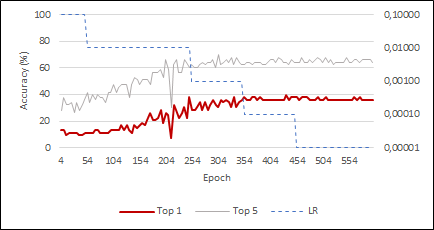
\includegraphics[width=0.5\textwidth]{images/results_20}
    \captionof{figure}{Accuracy obtained by the presented approach in recognition of the 20 signs selected from the ASLLVD.}
    \label{fig:training-asllvd-20}
    \end{center}
%\end{figure*}


\end{multicols}

%\vspace{-4mm}

To establish a reference to the complete ASLLVD dataset, a second experiment was performed using its 2,745 signs. In this scenario, an accuracy (\textit{top-1}) of 20.85\% and a \textit{top-5} accuracy of approximately 40.15\% was obtained. Of course, this is a much more challenging task than the one proposed in~\cite{lim-2016}, and these results reflect this complexity.

From the table, we can see that the approach presented in this paper, based on graphs of the coordinates of human articulations, has not yet been able to provide such remarkable results as that based on the description of the individual movement of the hands through histograms adopted by BHOF. Indeed, the application of consecutive steps for optical flow extraction, color map creation, block segmentation and generation of histograms from them were able to ensure that more enhanced features about the hand movements were extracted favoring its sign recognition performance. This technique is derived from HOF and differs only by the approach of focusing on the hands of individuals while calculating the optical flow histogram.

Methods such as MEI and MHI, however, present more primitive approaches, which mainly detect the movements and their intensity from the difference between the consecutive frames of actions. They are not able to differentiate individuals or to focus on specific parts of their body, causing movements of any nature considered equivalent. The PCA, in turn, adds the ability to reduce the dimensionality of the components based on the identification of those with greater variance and that, consequently, are more relevant for the detection of movement in the frames.

%%%%%%%%%%%%%%%%%%%%%%%%%%%%%%%%%%%%%%%%%%%%%%%%%%%%%%%%%%%%%%%%%%%%%%%%%
\section{Final remarks} 
\label{sec:final-remarks}

The results obtained with the presented approach did not reach such expressive performance as those obtained by some of the related techniques. However, its contributions are significant in guiding the next steps to be taken by future studies in this field.

Based on what is observed in this paper, it is relevant to seek approaches capable of enriching the information about the movements of the estimated coordinates, especially those of the hands and fingers, which, although very subtle, play a central role in the articulation and meaning of the signs.

This may be related, for example, to the definition of a new partitioning strategy that would allow more emphasis on the subtle traces of hands and fingers to the detriment of the other parts of the body. In addition, the definition of specific weights for these parts would enable the model to learn more about its dynamics; today the model does not distinguish the type of joint being learned. Finally, to include the depth information in the coordinates can provide the model with more details about the trajectory of the movement of these parts, enabling it to observe them through the three-dimensional plane.